% Options for packages loaded elsewhere
\PassOptionsToPackage{unicode}{hyperref}
\PassOptionsToPackage{hyphens}{url}
%
\documentclass[
  12pt,
  man, donotrepeattitle,floatsintext]{apa6}
\usepackage{amsmath,amssymb}
\usepackage{lmodern}
\usepackage{iftex}
\ifPDFTeX
  \usepackage[T1]{fontenc}
  \usepackage[utf8]{inputenc}
  \usepackage{textcomp} % provide euro and other symbols
\else % if luatex or xetex
  \usepackage{unicode-math}
  \defaultfontfeatures{Scale=MatchLowercase}
  \defaultfontfeatures[\rmfamily]{Ligatures=TeX,Scale=1}
  \setmainfont[]{Times New Roman}
\fi
% Use upquote if available, for straight quotes in verbatim environments
\IfFileExists{upquote.sty}{\usepackage{upquote}}{}
\IfFileExists{microtype.sty}{% use microtype if available
  \usepackage[]{microtype}
  \UseMicrotypeSet[protrusion]{basicmath} % disable protrusion for tt fonts
}{}
\makeatletter
\@ifundefined{KOMAClassName}{% if non-KOMA class
  \IfFileExists{parskip.sty}{%
    \usepackage{parskip}
  }{% else
    \setlength{\parindent}{0pt}
    \setlength{\parskip}{6pt plus 2pt minus 1pt}}
}{% if KOMA class
  \KOMAoptions{parskip=half}}
\makeatother
\usepackage{xcolor}
\usepackage{graphicx}
\makeatletter
\def\maxwidth{\ifdim\Gin@nat@width>\linewidth\linewidth\else\Gin@nat@width\fi}
\def\maxheight{\ifdim\Gin@nat@height>\textheight\textheight\else\Gin@nat@height\fi}
\makeatother
% Scale images if necessary, so that they will not overflow the page
% margins by default, and it is still possible to overwrite the defaults
% using explicit options in \includegraphics[width, height, ...]{}
\setkeys{Gin}{width=\maxwidth,height=\maxheight,keepaspectratio}
% Set default figure placement to htbp
\makeatletter
\def\fps@figure{htbp}
\makeatother
\setlength{\emergencystretch}{3em} % prevent overfull lines
\providecommand{\tightlist}{%
  \setlength{\itemsep}{0pt}\setlength{\parskip}{0pt}}
\setcounter{secnumdepth}{-\maxdimen} % remove section numbering
% Make \paragraph and \subparagraph free-standing
\ifx\paragraph\undefined\else
  \let\oldparagraph\paragraph
  \renewcommand{\paragraph}[1]{\oldparagraph{#1}\mbox{}}
\fi
\ifx\subparagraph\undefined\else
  \let\oldsubparagraph\subparagraph
  \renewcommand{\subparagraph}[1]{\oldsubparagraph{#1}\mbox{}}
\fi
\newlength{\cslhangindent}
\setlength{\cslhangindent}{1.5em}
\newlength{\csllabelwidth}
\setlength{\csllabelwidth}{3em}
\newlength{\cslentryspacingunit} % times entry-spacing
\setlength{\cslentryspacingunit}{\parskip}
\newenvironment{CSLReferences}[2] % #1 hanging-ident, #2 entry spacing
 {% don't indent paragraphs
  \setlength{\parindent}{0pt}
  % turn on hanging indent if param 1 is 1
  \ifodd #1
  \let\oldpar\par
  \def\par{\hangindent=\cslhangindent\oldpar}
  \fi
  % set entry spacing
  \setlength{\parskip}{#2\cslentryspacingunit}
 }%
 {}
\usepackage{calc}
\newcommand{\CSLBlock}[1]{#1\hfill\break}
\newcommand{\CSLLeftMargin}[1]{\parbox[t]{\csllabelwidth}{#1}}
\newcommand{\CSLRightInline}[1]{\parbox[t]{\linewidth - \csllabelwidth}{#1}\break}
\newcommand{\CSLIndent}[1]{\hspace{\cslhangindent}#1}
\ifLuaTeX
\usepackage[bidi=basic]{babel}
\else
\usepackage[bidi=default]{babel}
\fi
\babelprovide[main,import]{english}
% get rid of language-specific shorthands (see #6817):
\let\LanguageShortHands\languageshorthands
\def\languageshorthands#1{}
% Manuscript styling
\usepackage{upgreek}
\captionsetup{font=singlespacing,justification=justified}

% Table formatting
\usepackage{longtable}
\usepackage{lscape}
% \usepackage[counterclockwise]{rotating}   % Landscape page setup for large tables
\usepackage{multirow}		% Table styling
\usepackage{tabularx}		% Control Column width
\usepackage[flushleft]{threeparttable}	% Allows for three part tables with a specified notes section
\usepackage{threeparttablex}            % Lets threeparttable work with longtable

% Create new environments so endfloat can handle them
% \newenvironment{ltable}
%   {\begin{landscape}\centering\begin{threeparttable}}
%   {\end{threeparttable}\end{landscape}}
\newenvironment{lltable}{\begin{landscape}\centering\begin{ThreePartTable}}{\end{ThreePartTable}\end{landscape}}

% Enables adjusting longtable caption width to table width
% Solution found at http://golatex.de/longtable-mit-caption-so-breit-wie-die-tabelle-t15767.html
\makeatletter
\newcommand\LastLTentrywidth{1em}
\newlength\longtablewidth
\setlength{\longtablewidth}{1in}
\newcommand{\getlongtablewidth}{\begingroup \ifcsname LT@\roman{LT@tables}\endcsname \global\longtablewidth=0pt \renewcommand{\LT@entry}[2]{\global\advance\longtablewidth by ##2\relax\gdef\LastLTentrywidth{##2}}\@nameuse{LT@\roman{LT@tables}} \fi \endgroup}

% \setlength{\parindent}{0.5in}
% \setlength{\parskip}{0pt plus 0pt minus 0pt}

% Overwrite redefinition of paragraph and subparagraph by the default LaTeX template
% See https://github.com/crsh/papaja/issues/292
\makeatletter
\renewcommand{\paragraph}{\@startsection{paragraph}{4}{\parindent}%
  {0\baselineskip \@plus 0.2ex \@minus 0.2ex}%
  {-1em}%
  {\normalfont\normalsize\bfseries\itshape\typesectitle}}

\renewcommand{\subparagraph}[1]{\@startsection{subparagraph}{5}{1em}%
  {0\baselineskip \@plus 0.2ex \@minus 0.2ex}%
  {-\z@\relax}%
  {\normalfont\normalsize\itshape\hspace{\parindent}{#1}\textit{\addperi}}{\relax}}
\makeatother

% \usepackage{etoolbox}
\makeatletter
\patchcmd{\HyOrg@maketitle}
  {\section{\normalfont\normalsize\abstractname}}
  {\section*{\normalfont\normalsize\abstractname}}
  {}{\typeout{Failed to patch abstract.}}
\patchcmd{\HyOrg@maketitle}
  {\section{\protect\normalfont{\@title}}}
  {\section*{\protect\normalfont{\@title}}}
  {}{\typeout{Failed to patch title.}}
\makeatother

\usepackage{xpatch}
\makeatletter
\xapptocmd\appendix
  {\xapptocmd\section
    {\addcontentsline{toc}{section}{\appendixname\ifoneappendix\else~\theappendix\fi\\: #1}}
    {}{\InnerPatchFailed}%
  }
{}{\PatchFailed}
\usepackage{lineno}

\linenumbers
\usepackage{csquotes}
\usepackage[titles]{tocloft}
\cftpagenumbersoff{figure}
\renewcommand{\cftfigpresnum}{\itshape\figurename\enspace}
\renewcommand{\cftfigaftersnum}{.\space}
\setlength{\cftfigindent}{0pt}
\setlength{\cftafterloftitleskip}{0pt}
\settowidth{\cftfignumwidth}{Figure 10.\qquad}
\usepackage{float}
\floatplacement{figure}{H}
\usepackage{booktabs}
\raggedbottom
\usepackage{tabu}
\usepackage{makecell}
\usepackage{pdflscape}
\usepackage{longtable}
\newcommand{\blandscape}{\begin{landscape}}
\newcommand{\elandscape}{\end{landscape}}
\setlength\parindent{22pt}
\ifLuaTeX
  \usepackage{selnolig}  % disable illegal ligatures
\fi
\IfFileExists{bookmark.sty}{\usepackage{bookmark}}{\usepackage{hyperref}}
\IfFileExists{xurl.sty}{\usepackage{xurl}}{} % add URL line breaks if available
\urlstyle{same} % disable monospaced font for URLs
\hypersetup{
  pdfauthor={Emilio M. Bruna1,2,3, Maria Uriarte4, Maria Rosa Darrigo3, Paulo Rubim3, Cristiane F. Jurinitz3, Eric R. Scott1, Osmaildo Ferreira da Silva3, \& W. John Kress5},
  pdflang={en-EN},
  hidelinks,
  pdfcreator={LaTeX via pandoc}}

\title{\emph{METADATA FOR:}\\
\textbf{Demography of the understory herb \emph{Heliconia acuminata} (Heliconiaceae) in an experimentally fragmented tropical landscape}}
\author{Emilio M. Bruna\textsuperscript{1,2,3}, Maria Uriarte\textsuperscript{4}, Maria Rosa Darrigo\textsuperscript{3}, Paulo Rubim\textsuperscript{3}, Cristiane F. Jurinitz\textsuperscript{3}, Eric R. Scott\textsuperscript{1}, Osmaildo Ferreira da Silva\textsuperscript{3}, \& W. John Kress\textsuperscript{5}}
\date{}


\shorttitle{Metadata, Bruna et al.}

\authornote{

Correspondence concerning this article should be addressed to Emilio M. Bruna. E-mail: \href{mailto:embruna@ufl.edu}{\nolinkurl{embruna@ufl.edu}}

}

\affiliation{\vspace{0.5cm}\textsuperscript{1} Department of Wildlife Ecology and Conservation, University of Florida, PO Box 110430, Gainesville, FL 32611-0430, USA\\\textsuperscript{2} Center for Latin American Studies, University of Florida, PO Box 115530, Gainesville, FL 32611-5530, USA\\\textsuperscript{3} Biological Dynamics of Forest Fragments Project, INPA-PDBFF, CP 478, Manaus, AM 69011-970, Brazil\\\textsuperscript{4} Department of Ecology, Evolution and Environmental Biology, Columbia University, 1200 Amsterdam Ave., New York, New York 10027, USA\\\textsuperscript{5} Department of Botany, National Museum of Natural History, PO Box 37012, Smithsonian Institution, PO Box 37012, Washington DC, USA}

\note{

\emph{Open Research Statement}: Data are available as Supporting Information and are also available in Dryad at \url{https://doi.org/------}

\emph{Corresponding author}: Emilio M. Bruna (\href{mailto:embruna@ufl.edu}{\nolinkurl{embruna@ufl.edu}})

\newpage

}

\begin{document}
\maketitle

\hypertarget{metadata}{%
\section{METADATA}\label{metadata}}

\noindent  
\textbf{I. CLASS I. Data Set Descriptors}

\noindent
\textbf{A. Data set identity:} Demographic data from populations of the understory herb \emph{Heliconia acuminata} (Heliconiaceae) in an experimentally fragmented tropical landscape (1997-2009).

\noindent
\textbf{B. Data set identification code:}

\begin{enumerate}
\def\labelenumi{\arabic{enumi}.}
\tightlist
\item
  Data set File 1: \texttt{HDP\_plots.csv}\\
\item
  Data set File 2: \texttt{HDP\_1997\_2009.csv}
\end{enumerate}

\noindent
\textbf{C. Data set description:}

\begin{enumerate}
\def\labelenumi{\arabic{enumi}.}
\tightlist
\item
  \textbf{Originators:} Emilio M. Bruna, Department of Wildlife Ecology and Conservation, University of Florida, PO Box 110430, Gainesville, FL 32611-0430, USA and Center for Latin American Studies, University of Florida, PO Box 115530, Gainesville, FL 32611, USA.
\end{enumerate}

\begin{enumerate}
\def\labelenumi{\arabic{enumi}.}
\setcounter{enumi}{1}
\tightlist
\item
  \textbf{Abstract:} Habitat fragmentation is thought to be a leading cause of extinction, but the demography of species in fragmented landscapes remains poorly understood. This is particularly true in tropical ecosystems, where studies monitoring populations of species in both fragments and areas of continuous habitat across all life-history stages are virtually nonexistent. Here we report 12 years (1997-2009) of annual censuses of 13 populations of the Amazonian understory herb \emph{Heliconia acuminata} (LC Rich.). These surveys were conducted in plots established in the experimentally fragmented landscape of the Biological Dynamics of Forest Fragments Project, located north of Manaus, Brazil. The plots, each \(50\times100\)m, are located in forest fragments of different sizes (N = 4 plots in 1-ha fragments and N = 3 plots in 10-ha fragments) as well as continuous forest (N = 6 plots). The population in each plot was censused annually, at which time we recorded, identified, marked, and measured new seedlings, identified any previously marked plants that had died, and recorded the size of individuals that survived. During the flowering season we conducted regular surveys to recorded the identity of flowering plants and the number of inflorescences each produced. The resulting data set comprises \textgreater67000 plant\(\times\)year records of 8586 plants, including 3464 seedlings that became established after the initial census. These data have been used in publications on topics ranging from how fragmentation-related reductions in germination influence population dynamics to tests of statistical methods for analyzing reproductive rates (see \emph{Class V Supplemental Descriptors}, below) .
\end{enumerate}

\noindent
\textbf{D. Key words:} Amazon, Brazil, deforestation, demography, edge effects, flowering, forest fragments, habitat fragmentation, integral projection models, matrix models, population dynamics, vital rates.

\noindent 
\textbf{CLASS II. RESEARCH ORIGIN DESCRIPTORS}

\noindent  
\textbf{A. Overall project description:}

\begin{enumerate}
\def\labelenumi{\arabic{enumi}.}
\item
  \textbf{Identity:} The \emph{Heliconia} Demography Project
\item
  \textbf{Originators:} Emilio M. Bruna, W. John Kress, and María Uriarte
\item
  \textbf{Period of study:} 1997-2009
\item
  \textbf{Objectives:} Habitat fragmentation continues to be a major focus of research by ecologists (Didham et al. 2012, Haddad et al. 2015, Brudvig et al. 2017, Resasco et al. 2017, Fletcher et al. 2018) decades after it was first identified as a threat to the integrity of ecosystems (Harris 1984, Wilcove et al. 1986). A large body of empirical research has documented myriad biotic changes associated with fragmentation, including the local extinction of plant species from fragments (Harrison and Bruna 1999, Laurance et al. 2011). Although the demographic mechanisms underlying these extinctions are rarely known (Bruna et al. 2009), they are often hypothesized to result from reduced rates of individual growth, reproduction, or survivorship in fragments (Laurance et al. 1998, Zartman et al. 2015). This is especially true in tropical forest fragments, where abiotic conditions can be dramatically different from those in primary forest (reviewed in Broadbent et al. 2008). Tests of this hypothesis remain limited, however, by the paucity of long-term demographic data collected in both tropical forest fragments and continuous forest sites (Bruna et al. 2009).
\end{enumerate}

\begin{quote}
Most studies investigating the effects of forest fragmentation on tropical plants focus on trees (Cordeiro et al. 2009, Jurinitz et al. 2013, Zambrano and Salguero-Gómez 2014), in part because they are major reservoirs of carbon (Slik et al. 2010, Lasky et al. 2014). However, herbaceous species can comprise up to 30\% of the plant species in lowland tropical forests (Gentry and Emmons 1987, Ribeiro et al. 2010, Iannone and Vargas 2022, Spicer et al. 2022), where they are habitat and food for myriad animal taxa and economically and culturally vital non-timber forest products (Nakazono et al. 2004, Athayde et al. 2006). Despite their biocultural importance, however, the way in which habitat fragmentation and other global change phenomena influences the population dynamics of tropical understory plants remains conspicuously understudied (Bruna et al. 2009).
\end{quote}

\begin{quote}
The \emph{Heliconia} Demography Project (HDP) was established to address the lack of data on the demography of understory plants in fragmented tropical landscapes. The core of the HDP is annual censuses of thirteen populations of \emph{Heliconia acuminata} located in either continuous forest or experimentally isolated forest fragments at Brazil's Biological Dynamiocs of Forest Fragments Project (Laurance et al. 2011) The primary purpose behind their initial collection was to parameterize size-structured demographic models (Caswell 2000, Ellner and Rees 2006) with which to (1) compare the demography and population dynamics of \emph{H. acuminata} populations in fragments and continuous forest, and (2) test the hypothesis that reductions in seedling establishment in forest fragments would lead to population declines.
\end{quote}

\begin{enumerate}
\def\labelenumi{\arabic{enumi}.}
\setcounter{enumi}{4}
\item
  \textbf{Abstract:} Here we report 12 years (1997-2009) of annual censuses of 13 populations of the Amazonian understory herb \emph{Heliconia acuminata} (LC Rich.). These surveys were conducted in plots established in the experimentally fragmented landscape of the Biological Dynamics of Forest Fragments Project, located north of Manaus, Brazil. The plots, each \(50\times100\)m, are located in forest fragments of different sizes (N = 4 plots in 1-ha fragments and N = 3 plots in 10-ha fragments) as well as continuous forest (N = 6 plots). The population in each plot was censused annually, at which time we recorded identified, marked, and measured new seedlings, identified any previously marked plants that had died, and recorded the size of individuals that survived. During the flowering season we conducted regular surveys to recorded the identity of flowering plants and the number of inflorescences each produced. The resulting data set comprises \textgreater67000 plant\(\times\)year records of N = 8586 plants, including N = 3464 seedlings that became established after the initial census. These data have been used in publications on topics ranging from how fragmentation-related reductions in germination influence population growth rates to tests of statistical methods for analyzing reproductive rates.
\item
  \textbf{Sources of funding:} The initial establishment of plots and the 1997-2002 surveys were supported by grants to E. M. Bruna from the Smithsonian Institution (Graduate Student Research Award), the University of California, Davis (Center for Population Biology Graduate Research Grant, M. E. Mathias Graduate Research Grant), the Biological Dynamics of Forest Fragments Project (Graduate Student Logistics Grant), the National Science Foundation (Dissertation Improvement Grant INT 98-06351), and the Ford Foundation (Dissertation Year Fellowship). The 2001-2005 surveys were supported a grant from the National Science Foundation to E. M. Bruna (Research Starter Grant DEB-0309819). The 2006-2009 surveys were supported by grants from the National Science Foundation to E. M. Bruna (DEB-0614149) and María Uriarte (DEB-0614339). Subsequent analyses and the preparation of these data for archiving were supported by the National Science Foundation (DEB-1948607).
\end{enumerate}

\noindent  
\textbf{B. Subproject description}

\begin{enumerate}
\def\labelenumi{\arabic{enumi}.}
\tightlist
\item
  \textbf{Site description}
\end{enumerate}

\begin{quote}
\begin{enumerate}
\def\labelenumi{\alph{enumi}.}
\tightlist
\item
  \textbf{Site type:} Lowland tropical forest
\end{enumerate}
\end{quote}

\begin{quote}
\begin{enumerate}
\def\labelenumi{\alph{enumi}.}
\setcounter{enumi}{1}
\tightlist
\item
  \textbf{Geography:} The data were collected at the Biological Dynamics of Forest Fragments Project (BDFFP, 2°30'S, 60°W), a 1000-km mosaic of lowland forest, forest fragments, secondary forests, and pastures located approximately 70 km north of Manaus, Amazonas, Brazil (Fig. 1).
\end{enumerate}
\end{quote}

\begin{quote}
\begin{enumerate}
\def\labelenumi{\alph{enumi}.}
\setcounter{enumi}{2}
\tightlist
\item
  \textbf{Habitat:} The BDFFP is dominated by tropical evergreen lowland forest (i.e., `tropical moist forest', \emph{sensu} Holdridge (1967). The forest canopy at the sites is \textasciitilde35--40 m tall, with emergent trees of up to \textasciitilde45 m (Rankin-de-Mérona et al. 1992). The tree community at the BDFFP is highly diverse: \textasciitilde1300 species total (Laurance 2001), with as many as 280 tree species ha\(^-\)\(^1\) (Oliveira and Mori 1999). The understory is dominated by stemless palms (Scariot 1999). All HDP plots are located in \emph{terra-firme} (i.e., non-flooded) forest and none are bisected by streams.
\end{enumerate}
\end{quote}

\begin{quote}
\begin{enumerate}
\def\labelenumi{\alph{enumi}.}
\setcounter{enumi}{3}
\tightlist
\item
  \textbf{Geology:} Soils in the sites are nutrient-poor xanthic ferralsols, known as yellow latosols in the Brazilian soil classification system. Despite their high clay content they have poor water-retention capacity (Fearnside and Leal-Filho 2001). The often rugged topography at the BDFFP ranges in elevation from 50-150 m elevation (Gascon and Bierregaard 2001).
\end{enumerate}
\end{quote}

\begin{quote}
\begin{enumerate}
\def\labelenumi{\alph{enumi}.}
\setcounter{enumi}{4}
\tightlist
\item
  \textbf{Watersheds:} The BDFFP landscape includes catchments of the Urubu, Cuieiras, and Preto da Eva rivers (Nessimian et al. 2008).
\end{enumerate}
\end{quote}

\begin{quote}
\begin{enumerate}
\def\labelenumi{\alph{enumi}.}
\setcounter{enumi}{5}
\tightlist
\item
  \textbf{Site history:} A complete history of the BDFFP can be found in Gascon and Bierregaard (2001) and Bierregaard et al. (2002). Briefly, the BDFFP reserves were established on three cattle ranches. Fragments were isolated between 1980-1984 by felling the trees surrounding the patch of forest to be isolated (Lovejoy et al. 1986). Fragment reserves were fenced to prevent the incursion of cattle from the surrounding pastures. To ensure fragments remain isolated, a 100m strip around each fragment is regularly cleared of the secondary growth (Gascon and Bierregaard 2001). The structure and species composition of the secondary growth that surrounds a fragment, which is strongly dependent on whether fire was used to clear land prior to planting pasture grasses (Mesquita et al. 2001), can have large effects on the species composition, ecological processes, and abiotic conditions in fragments (reviewed in Laurance et al. 2002, 2011). The BDFFP is currently administered collaboratively by the Smithsonian Tropical Research Institute and Brazil's Instituto Nacional de Pesquisas da Amazônia (INPA).
\end{enumerate}
\end{quote}

\begin{quote}
\begin{enumerate}
\def\labelenumi{\alph{enumi}.}
\setcounter{enumi}{6}
\tightlist
\item
  \textbf{Climate:} Mean annual temperature at the site is 26\(^\circ\)C (range 19-39\(^\circ\)C). Annual rainfall ranges from 1900-2300 mm (Scott et al. 2022), with a pronounced dry season from June-December in which there is \textless100 mm rain per month.
\end{enumerate}
\end{quote}

\begin{enumerate}
\def\labelenumi{\arabic{enumi}.}
\setcounter{enumi}{1}
\tightlist
\item
  \textbf{Sampling Design}
\end{enumerate}

\begin{quote}
\begin{enumerate}
\def\labelenumi{\alph{enumi}.}
\tightlist
\item
  \textbf{Design characteristics}: Annual demographic surveys of \emph{Heliconia acuminata} populations were carried out in 13 permanent plots distributed across the BDFFP landscape (Bruna and Kress 2002). Six plots are located in continuous forest, four in 1-ha fragments, and three in 10-ha fragments (one plot per fragment; Fig. 1).
\end{enumerate}
\end{quote}

\begin{quote}
\begin{quote}
\emph{Heliconia acuminata} (Heliconiaceae) is a perennial, self-incompatible monocot native to Amazonia (Kress 1990) and widely distributed throughout the Amazon basin (Kress 1990). Although many species of \emph{Heliconia} grow in large aggregations on roadsides, gaps, and in other disturbed habitats, others, including \emph{H. acuminata}, grow primarily in the shaded forest understory (Kress 1983). \emph{Heliconia acuminata} is the most abundant understory herb throughout much of the BDFFP (Ribeiro et al. 2010); the other two \emph{Heliconia} species found in the BDFFP reserves are either very rare (\emph{H. latispatha}) and restricted saturated soils adjacent to streams (\emph{H. tarumaensis}).
\end{quote}
\end{quote}

\begin{quote}
\begin{quote}
Each \emph{Heliconia acuminata} has a basal rhizome from which emerge erect vegetative shoots with broad leaves. Reproductive plants have one or more flowering shoots, each of which has a single infloresence. Plants grow slowly (Bruna and Ribeiro 2005, Gagnon et al. 2011) and the proportion of plants that flower is low (Bruna 2002, Bruna and Kress 2002). The primary herbivores of \emph{Heliconia} species are Hispine beetles, whose larvae and adults scrape the surface of unrolled immamture leaves (Strong 1977). The beetle species associated with \emph{H. acuminata} is \emph{Cephaloleia nigriceps} Baly (Staines and Garcia-Robledo 2014); it actually does little damage to leaves but can cause extensive damage to bracts, flowers, and developing ovaries.
\end{quote}
\end{quote}

\begin{quote}
\begin{quote}
\emph{Heliconia} can be propagated by segmenting the rhizome (Berry and Kress 1991, Bruna and Andrade 2011), and clonal spread is common in the \emph{Heliconia} species found in open or disturbed habitats (Schleuning et al. 2008). However, recruitment in \emph{H. acuminata} and other understory species is primarily via seeds (Bruna 1999, 2002). Plants that flower do so during the rainy season, with the propbability of flowering increasing with plant size (Bruna and Kress 2002). The overwhelming majority of plants in our data set that flowered (75\%) produced a single infloresence (range = 1-7). Infloresences have an average 22.28 ± 1.17 SE flowers (range 4-62); each flower remains open for one day before falling from the plant. Pollen transfer experiments indicate self-compatibility is extremely low (Bruna and Darrigo, \emph{unpubl. data}); succesfully pollinated flowers can produce 1-3 seeds, with an average of 2 seeds per fruit (Bruna 2014).
\end{quote}
\end{quote}

\begin{quote}
\begin{quote}
\emph{Heliconia acuminata} is pollinated by the `traplining' hummingbirds \emph{Phaeothornis superciliosus} and \emph{P. bourcieri}. Visitation rates to flowers are extremely low (\textless1 visit hour\textsuperscript{-1}, Bruna et al. 2004), as are rates of fruit production (Bruna and Kress 2002). The fleshy blue fruits are consumed by birds (Uriarte et al. 2011); in our study sites the primary dispersers are the White-necked Thrush (\emph{Turdus albicollis}), the Thrush-like-Manakin (\emph{Schiffornis turdinus}), and several species of manakin (\emph{Pipra erythrocephala}, \emph{P. pipra}, \emph{Lepidothrix serena}, and \emph{Corapipo gutturalis}). The seeds germinate 6-7 months after dispersal, which coincides with the onset of the rainy season (Bruna 1999, 2002). Experiments indicate that post-dispersal seed predation is negligible and while rates of seed germination and seedling establishment were generally low, they were significantly higher in continuous forest than forest fragments (Bruna 1999, 2002). Although some seeds germinated \textgreater1 year after experimental dispersal, this was generally rare - especially in fragments. These results are consistent with the generalization that few plant species in lowland tropical forests have long-lived seed banks (Vázquez-Yanes and Orozco-Segovia 1993).
\end{quote}
\end{quote}

\begin{quote}
\begin{enumerate}
\def\labelenumi{\alph{enumi}.}
\setcounter{enumi}{1}
\tightlist
\item
  \textbf{Permanent Plots:} Each demographic plot is \(50\times100\)m and is subdivided into 50 contiguous subplots of \(10\times10\)m to facilitate the surveys. Plots in 1-ha fragments were established in a randomly selected half of the fragment (Fig. 2), plots in 10-ha fragments are located in the center of the fragment (Fig. 3), and plots in continuous forest are located 500-4000 m from any borders with cattle pastures or secondary forest (Fig. 4). The plots furthest apart are from each other are separated by \textasciitilde70 km.
\end{enumerate}
\end{quote}

\begin{quote}
\begin{quote}
Plots in 1-ha fragments, 10-ha fragments, and three of the continuous forest sites were demarcated in January-April 1997. The remaining three plots in continuous forest were demarcated in January 1998, which was also when the first complete census in all plots was conducted. To mark the plants, a team of 2-3 people slowly walked through each subplot and located all \emph{Heliconia acuminata} and marked them with a wooden stake to which was attached an individually numbered aluminum tag. The size of each plant was measured in two ways: (1) by counting its number of vegetative shoots and (2) by measuring the height of the plant from the ground to the top of its highest leaf (rounded to the nearest cm). Three additional plots were established in continuous forest sites in 1998 (CF 4-6); all plants in these plots were tagged and measuring in the same way as in other plots.
\end{quote}
\end{quote}

\begin{quote}
\begin{enumerate}
\def\labelenumi{\alph{enumi}.}
\setcounter{enumi}{2}
\tightlist
\item
  \textbf{Frequency of Data Collection:} Plots were censused annually at the onset of the rainy season to coincide with seedling establishment (generally late January to February). The exception to this was the three continuous forest plots established in August 1998, which were censused in August 1999. Regular visits were made to all 13 plots throughout the rainy season to identify reproductive individuals and record the number of flowering shoots (i.e., infloresences) that they had produced.
\end{enumerate}
\end{quote}

\begin{enumerate}
\def\labelenumi{\arabic{enumi}.}
\setcounter{enumi}{2}
\tightlist
\item
  Research Methods
\end{enumerate}

\begin{quote}
\begin{enumerate}
\def\labelenumi{\alph{enumi}.}
\tightlist
\item
  \textbf{Demographic Surveys:} During each census team members recorded which plants died, the size (i.e., height and number of shoots) of all surviving plants, and the size of all new seedlings, which were also marked with a numbered tag. Survey team members also noted any new canopy gaps created by fallen trees or limbs, estimated the proportion of any suplot that was affected by a treefall (available at the HDP Github repository: \url{https://github.com/BrunaLab/HeliconiaSurveys}), and recorded if plants were under treefalls or damaged by fallen branches or palm fronds.
\end{enumerate}
\end{quote}

\begin{quote}
\begin{enumerate}
\def\labelenumi{\alph{enumi}.}
\setcounter{enumi}{1}
\tightlist
\item
  \textbf{Taxonomy and systematics:} \emph{Heliconia} is the only genus in the family Heliconiaceae. This family is distinguished from the others in the order Zingiberales by having inverted flowers, a single staminode, and drupaceous fruits (Kress 1990). It is estimated that there are 200-250 species of \emph{Heliconia}, almost all of which are native to the Neotropics. \emph{Heliconia acuminata} L. C. (Rich.) (Richard 1831) is one of the approximately 20 \emph{Heliconia} species found in the Brazilian Amazon (Kress 1990). We deposited voucher specimens of \emph{H. acuminata} collected in areas adjacent to demographic plots at the herbaria of the Instituto Nacional de Pesquisas da Amazônia (Accession Numbers INPA 189569-189573) and the University of California, Davis (Accession Numbers DAV 69391-69396).
\end{enumerate}
\end{quote}

\begin{enumerate}
\def\labelenumi{\arabic{enumi}.}
\setcounter{enumi}{3}
\tightlist
\item
  \textbf{Project personnel:} In addition to the Originators, other key personnel include the Project Managers that were responsible for coordinating the annual censuses and other field activities, BDFFP Technicians (\emph{``Mateiros''}) that assisted with data collection and provided logistical support in the field, and undergraduate and postgraduate field assistants hired to assist with the surveys.
\end{enumerate}

\begin{quote}
\begin{enumerate}
\def\labelenumi{\alph{enumi}.}
\tightlist
\item
  \textbf{Project Managers:} Paulo Rubim (2007-2012), Maria Beatriz Nogueira (2002), Maria Rosa Darrigo (2002-2003), Cris Follman Jurinitz (2003), Simone Benedet (2004).
\end{enumerate}
\end{quote}

\begin{quote}
\begin{enumerate}
\def\labelenumi{\alph{enumi}.}
\setcounter{enumi}{1}
\tightlist
\item
  \textbf{BDFFP Technicians:} Osmaildo Ferreira da Silva, Francisco Marques, Alaercio Marajó dos Reis, João de Deus Fragata, Romeu Cardoso.
\end{enumerate}
\end{quote}

\begin{quote}
\begin{enumerate}
\def\labelenumi{\alph{enumi}.}
\setcounter{enumi}{2}
\tightlist
\item
  \textbf{Undergraduate \& Postgraduate Field Assistants:} Olavo Nardy (2000), Obed Garcia (2001), Sylvia Heredia (2001-2002), Maria Beatriz Nogueira (2002), Cris Follman Jurinitz (2003), David M. Lapola (2003), Denise Cruz (2003), Cristina Escate (2004), Bruno Turbiani (2005), Elisabete Marques da Costa (2006), Wesley Dáttilo da Cruz (2007), Jefferson José Valsko da Silva (2007).
\end{enumerate}
\end{quote}

\noindent  
\textbf{CLASS III. DATA SET STATUS AND ACCESSIBILITY}

\noindent  
\textbf{A. Status}

\begin{enumerate}
\def\labelenumi{\arabic{enumi}.}
\item
  \textbf{Latest update:}
\item
  \textbf{Latest archive date:} {[}\emph{date of archiving at Dryad to be added upon acceptance}{]}
\item
  \textbf{Metadata status:} Complete (last update:
  NA)
\item
  \textbf{Data verification:} An extensive review of the data was also conducted in preparation for archiving. We began by generating a list of potential anomalies that could indicate errors (e.g.~extremely large changes in size from one year to the next, plants marked as dead that had subsequent measurements), and then wrote code to search for these anomalies using the R statistical programming language (Team 2014). We also used the \texttt{pointblank} library (Iannone and Vargas 2022), which similarly identifies cases in a data set for review and validation. All records flagged were evaluated by E. M. Bruna by checking the values in the electronic records against the original data sheets. Corrections to the data set were also made using R scripts; the code documenting and implementing these changes is archived at Zenodo {[}\emph{url to be added upon acceptance}{]}. Questions regarding the data set or code should be referred to E. M. Bruna, who will investigate and update the database or code as needed. Code for any post-publication updates is maintained at the \href{https://github.com/BrunaLab/HeliconiaSurveys}{HDP Github Repository}.
\end{enumerate}

\noindent 
\textbf{B. Accessibility}

\begin{enumerate}
\def\labelenumi{\arabic{enumi}.}
\item
  \textbf{Storage location and medium:} Ecological Society of America Data Archives {[}url to be added{]} and the Dryad Digital Repository {[}url to be added{]}.
\item
  \textbf{Contact person:} Emilio M. Bruna, Department of Wildlife Ecology and Conservation, Box 110430, Gainesville, FL 32611 USA. Phone: (352) 846-0634. Email: \href{mailto:embruna@ufl.edu}{\nolinkurl{embruna@ufl.edu}}
\item
  \textbf{Copyright restrictions:} None
\item
  \textbf{Proprietary restrictions:} None.
\end{enumerate}

\begin{quote}
\begin{enumerate}
\def\labelenumi{\alph{enumi}.}
\tightlist
\item
  \textbf{Conditions of Reuse:} Any publication using data collected at the BDFFP must include a BDFFP Technical Series Number in the Acknowledgments. Authors can request this series number upon the acceptance of their article by contacting the BDFFP's Scientific Coordinator or E. M. Bruna.
\end{enumerate}
\end{quote}

\begin{quote}
\begin{enumerate}
\def\labelenumi{\alph{enumi}.}
\setcounter{enumi}{1}
\tightlist
\item
  \textbf{Citation:} Authors of any publications or products using these data should cite both this data paper and the Dryad data archive {[}\emph{citation of Dryad archive to be added upon acceptance}{]}. We also request that they provide E. M. Bruna a copy of their article upon acceptance, which allows us to track the data set's usage, inform users of any corrections or updates, report articles using the data to the funding agencies that provided support, and document the different ways in which the scientific community uses the data.
\end{enumerate}
\end{quote}

\begin{quote}
\begin{enumerate}
\def\labelenumi{\alph{enumi}.}
\setcounter{enumi}{2}
\tightlist
\item
  \textbf{Disclaimers:} While the data are provided in good faith and are accurrate to the best of our knowledge, they are provided ``as is''. We do not assume any legal liability or responsibility for their accuracy, completeness, or utility. The responsibility for use and analysis of these data lies completely with the user.
\end{enumerate}
\end{quote}

\begin{enumerate}
\def\labelenumi{\arabic{enumi}.}
\setcounter{enumi}{4}
\tightlist
\item
  \textbf{Costs of acquiring data:} None.
\end{enumerate}

\noindent  
\textbf{CLASS IV. DATA STRUCTURAL DESCRIPTORS}

\noindent  
\textbf{A. Data set File 1:} Descriptors of demographic plots

\begin{enumerate}
\def\labelenumi{\arabic{enumi}.}
\item
  \textbf{Identity:} \texttt{HDP\_plot\_descriptors.csv}
\item
  \textbf{Size:} 14 rows (including header), 404 Bytes
\item
  \textbf{Format and storage mode:} ASCII text, comma delimited. No
  compression scheme used.
\item
  \textbf{Header information:} The first row of the file contains the variable names.
\item
  \textbf{Alphanumeric attributes:} Mixed
\item
  \textbf{Special Characters:} Missing values are represented with NA.
\item
  \textbf{Authentication Procedures}: checksum (MD5:2d3ec96006667abab1ecc14e72055850)
\item
  \textbf{Start \& End Columns:} Start: \texttt{plot}, End: \texttt{yr\_isolated}
\item
  \textbf{Variable Information:} Each row is one plot, with the columns providing plot-specific values for each variable (Table 1).
\end{enumerate}

--\textgreater{}

\noindent 
\textbf{B. Data set File 2:} \emph{Heliconia} Demographic Data

\begin{enumerate}
\def\labelenumi{\arabic{enumi}.}
\item
  \textbf{Identity:} \texttt{HDP\_data\_1997-2009.csv}
\item
  \textbf{Size:} 66785 rows (including header), 3.61 MB
\item
  \textbf{Format and storage mode:} ASCII text, comma delimited. No compression scheme used.
\item
  \textbf{Header information:} The first row of the file contains the variable names.
\item
  \textbf{Alphanumeric attributes:} Mixed.
\item
  \textbf{Special Characters:} Missing values are represented with NA.
\item
  \textbf{Authentication Procedures}: Checksum (MD5:15bbb4869fe192649e93d3474d3145d1)
\item
  \textbf{Start \& End Columns:} Start: \texttt{plot}, End: \texttt{tag\_number}
\item
  \textbf{Data anomalies:} Plants that could not be found during a survey were recorded as `missing' but maintained on the survey list to be searched for in subsequent years. The same is true of plants under branches or the crowns of fallen trees, which might not be found for several years when the crown's leaves dried and fell or the area under the crown could be safely searched. The codes used to denote such cases are defined in Table 2.
\end{enumerate}

\begin{quote}
The stakes and numbered tags used to mark plants were sometimes displaced, broken, or buried under leaf litter as a result of tree falls or other disturbances. If a plant's tag couldn't be found after an extensive search, it would be marked with a new tag. In some cases, it was straightforward to determine such a plant's original number when entering the survey data (e.g., when all plants in a low-density subplot were found except one, which in the prior year was similar in size as the plant found without a tag). In those cases, the plant's prior measurements were transferred to the new number and we logged the details of the change in tag number; the log is available at the \href{https://github.com/BrunaLab/HeliconiaSurveys}{HDP Github repository}. In other cases, it was impossible to definitively determine a plant's original number (e.g., when two similarly sized plants in a subplots were both missing their tags). In these cases the original number was maintained in the database with the plant's status noted as `missing' in subsequent surveys. The record for the new number indicates the plant with which it is associated is an established plant that was found without a tag (see Section IV, Table 2) and not a new seedling.
\end{quote}

\begin{quote}
There were also cases in which established plants were found without tags in subplots where all previously tagged plants had already been located and measured, indicating previous survey teams had failed to find and mark them. These plants were marked, measured, and added to the database with a code indicating they were a established (i.e., post-seedling) but previously unmarked plant (See Table 2). Of the N = 947 plants in the data set, 11\% were found without tags after the plot had been established. Almost half of these (49\%) were in the three plots where \emph{H. acuminata} density was highest (CF-1, FF-7, CF-3).
\end{quote}

\begin{quote}
Due to logistical or financial constraints, no surveys were conducted in plot CF-6 in 2003, in plots CF-4, CF-5, and CF-6 in 2000, or plots FF-5,FF-6, and FF-7 in 2008-2009.
\end{quote}

\begin{enumerate}
\def\labelenumi{\arabic{enumi}.}
\setcounter{enumi}{7}
\tightlist
\item
  \textbf{Variable information:} Each row in the data set is a demographic plot, with columns of data describing that plot (Table 2). Blanks do not denote missing information, but rather nothing relevant to report.
\end{enumerate}

--\textgreater{}

\noindent
\textbf{CLASS V. SUPPLEMENTAL DESCRIPTORS}

\noindent  
\textbf{A. Data acquisition:}

\begin{enumerate}
\def\labelenumi{\arabic{enumi}.}
\item
  \textbf{Data forms:} Examples of the forms used to collect survey data are available on the \href{https://github.com/BrunaLab/HeliconiaSurveys}{HDP Github repository}.
\item
  \textbf{Location of original data forms, electronic files, and archived copies:} Original data sheets are stored at the University of Florida. Scanned copies of the data sheets (in .pdf format) and the electronic copies of the data in (in .csv format) are stored on a desktop computer at the University of Florida that is backed up daily to two portable hard drives and two cloud storage services. The integrity of digital files is verified semi-annually.
\item
  \textbf{Data entry verification procedures:} Following each survey, the measurements of plant height and stem number were compared with those from the previous year to identify potential errors in either plant measurement or entry (e.g., a plant with 1 shoot in year t and 11 shoots in year t+1 is likely an error in data entry). Discrepancies were investigated by referring to the original data sheets and, on occasion, returning to the field to remeasure plants.
\end{enumerate}

\noindent
\textbf{B. Quality assurance/quality control procedures:} An extensive review of the data was conducted in preparation for archiving. We began by generating a list of potential anomalies that could indicate errors (e.g.~extremely large changes in size from one year to the next, plants marked as dead that had subsequent measurements), and then wrote code to search for these anomalies using the R statistical programming language (Team 2014). We also used the \texttt{pointblank} library (Iannone and Vargas 2022), which similarly identifies cases in a data set for review and validation. All records flagged were evaluated by E. M. Bruna by checking the values in the electronic records against the original data sheets. Corrections to the data set were also made using R scripts; the code documenting and implementing these changes is archived at Zenodo {[}\emph{url to be added upon acceptance}{]}. Questions regarding the data set or code should be referred to E. M. Bruna, who will investigate and update the database or code as needed. Code for any post-publication updates is maintained at the \href{https://github.com/BrunaLab/HeliconiaSurveys}{HDP Github Repository}.

\noindent
\textbf{C. Related materials:} A diagram showing each demographic plots' location, orientation, and subdivision into subplots can be found in Appendix S1. Photographs, data summaries, updates, and other related materials can be found at the \href{https://github.com/BrunaLab/HeliconiaSurveys}{HDP Github Repository}.

\noindent
\textbf{D. Computer programs and data-processing algorithms:} The version of the R code used to prepare this data archive can be found at Zenodo {[}\emph{url to be added}{]}. Any post-publication updates to the code or data can be found at the HDP Github Repository (\url{https://github.com/BrunaLab/HeliconiaSurveys}).

\noindent
\textbf{F. Publications:}

\begin{enumerate}
\def\labelenumi{\arabic{enumi}.}
\tightlist
\item
  \textbf{Publications including analyses of the data set.} An update list and downloadable \emph{BibTeX} file can be found at the \href{https://github.com/BrunaLab/HeliconiaSurveys}{HDP Github repository}.
\end{enumerate}

\begin{quote}
\begin{enumerate}
\def\labelenumi{\arabic{enumi}.}
\tightlist
\item
  Bruna, E. M. and W. J. Kress. 2002. Habitat fragmentation and the demographic structure of an Amazonian understory herb (\emph{Heliconia acuminata}). \emph{Conservation Biology}, 16(5): 1256-1266.
\end{enumerate}
\end{quote}

\begin{quote}
\begin{enumerate}
\def\labelenumi{\arabic{enumi}.}
\setcounter{enumi}{1}
\tightlist
\item
  Bruna, E. M., O. Nardy, S. Y. Strauss, and S. P. Harrison. 2002. Experimental assessment of \emph{Heliconia acuminata} growth in a fragmented Amazonian landscape. \emph{Journal of Ecology}, 90(4): 639-649.
\end{enumerate}
\end{quote}

\begin{quote}
\begin{enumerate}
\def\labelenumi{\arabic{enumi}.}
\setcounter{enumi}{2}
\tightlist
\item
  Bruna, E. M. 2002. Effects of forest fragmentation on \emph{Heliconia acuminata} seedling recruitment in the central Amazon. \emph{Oecologia}, 132:235-243.
\end{enumerate}
\end{quote}

\begin{quote}
\begin{enumerate}
\def\labelenumi{\arabic{enumi}.}
\setcounter{enumi}{3}
\tightlist
\item
  Bruna, E. M. 2003. Are plant populations in fragmented habitats recruitment limited? Tests with an Amazonian herb. \emph{Ecology}, 84(4): 932-947.
\end{enumerate}
\end{quote}

\begin{quote}
\begin{enumerate}
\def\labelenumi{\arabic{enumi}.}
\setcounter{enumi}{4}
\tightlist
\item
  Bruna, E. M. 2004. Biological impacts of deforestation and fragmentation. Pages 85-90 in \emph{The Encyclopaedia of Forest Sciences}. J. Burley, J Evans, and J Youngquist, (eds.). Elsevier Press, London.
\end{enumerate}
\end{quote}

\begin{quote}
\begin{enumerate}
\def\labelenumi{\arabic{enumi}.}
\setcounter{enumi}{5}
\tightlist
\item
  Bruna, E. M., and M. K. Oli. 2005. Demographic effects of habitat fragmentation on a tropical herb: Life-table response experiments. \emph{Ecology} 86:1816-1824.
\end{enumerate}
\end{quote}

\begin{quote}
\begin{enumerate}
\def\labelenumi{\arabic{enumi}.}
\setcounter{enumi}{6}
\tightlist
\item
  Bruna E. M. \& W. J. Kress. 2005. Forest fragments and plant reproduction in Amazonian Brazil. pp.~141-146 in G. A. Krupnick \& W. J. Kress (eds). \emph{Plant conservation: a natural history approach}. University of Chicago Press, Chicago.
\end{enumerate}
\end{quote}

\begin{quote}
\begin{enumerate}
\def\labelenumi{\arabic{enumi}.}
\setcounter{enumi}{7}
\tightlist
\item
  Morris, W. F., C. A. Pfister, S. Tuljapurkar, C. V. Haridas, C. Boggs, M. S. Boyce, E. M. Bruna, D. R. Church, T. Coulson, D. F. Doak,, S. Forsyth, J-M. Gaillard, C. C. Horvitz, S. Kalisz, B. E. Kendall, T. M. Knight, C. T. Lee, and E. S. Menges. 2008. Longevity can buffer plant and animal populations against changing climatic variability. \emph{Ecology} 89(1): 19-25.
\end{enumerate}
\end{quote}

\begin{quote}
\begin{enumerate}
\def\labelenumi{\arabic{enumi}.}
\setcounter{enumi}{8}
\tightlist
\item
  Fiske, I., E. M. Bruna, and B. M. Bolker. 2008. Effect of sample size on estimates of population growth rates calculated with matrix models. \emph{PLoS ONE} 3(8): e3080.
\end{enumerate}
\end{quote}

\begin{quote}
\begin{enumerate}
\def\labelenumi{\arabic{enumi}.}
\setcounter{enumi}{9}
\tightlist
\item
  Fiske, I. and E. M. Bruna. 2010. Alternative spatial sampling in studies of plant demography: consequences for estimates of population growth rate. \emph{Plant Ecology} 207(2): 213-225.
\end{enumerate}
\end{quote}

\begin{quote}
\begin{enumerate}
\def\labelenumi{\arabic{enumi}.}
\setcounter{enumi}{10}
\tightlist
\item
  Uriarte, M., E. M. Bruna, P. Rubim, M. Anciaes, and I. Jonckeeere. 2010. Effects of forest fragmentation on seedling recruitment of an understory herb: assessing seed vs.~safe-site limitation. \emph{Ecology} 91(5):1317-1328.
\end{enumerate}
\end{quote}

\begin{quote}
\begin{enumerate}
\def\labelenumi{\arabic{enumi}.}
\setcounter{enumi}{11}
\tightlist
\item
  Gagnon, P. R., E. M. Bruna, P. Rubim, M. R. Darrigo, R. C. Littlel, M. Uriarte, and W. J. Kress. 2011. The growth of an understory herb is chronically reduced in Amazonian forest fragments. \emph{Biological Conservation} 144: 830-835.
\end{enumerate}
\end{quote}

\begin{quote}
\begin{enumerate}
\def\labelenumi{\arabic{enumi}.}
\setcounter{enumi}{12}
\tightlist
\item
  Uriarte, M. Anciães, M. T.B. da Silva, P. Rubim, E. Johnson, and E. M. Bruna. 2011. Disentangling the drivers of reduced long-distance seed dispersal by birds in an experimentally fragmented landscape. \emph{Ecology} 92(4): 924-93.
\end{enumerate}
\end{quote}

\begin{quote}
\begin{enumerate}
\def\labelenumi{\arabic{enumi}.}
\setcounter{enumi}{13}
\tightlist
\item
  Côrtes, M., M. Uriarte, M. Lemes, R. Gribel, W. J. Kress, P. Smouse, E. M. Bruna. 2013. Low plant density enhances gene flow in the Amazonian understory herb \emph{Heliconia acuminata}. \emph{Molecular Ecology} 22: 5716-5729.
\end{enumerate}
\end{quote}

\begin{quote}
\begin{enumerate}
\def\labelenumi{\arabic{enumi}.}
\setcounter{enumi}{14}
\tightlist
\item
  Brooks, M. E., K. Kristensen, M. R. Darrigo, P. Rubim, M. Uriarte, E. M. Bruna, and B. M Bolker. 2019. Statistical modeling of patterns in annual reproductive rates. \emph{Ecology} 100(7): e02706.
\end{enumerate}
\end{quote}

\begin{quote}
\begin{enumerate}
\def\labelenumi{\arabic{enumi}.}
\setcounter{enumi}{15}
\tightlist
\item
  Leite, MCA, R. Sauchuk, F.B. Agusto, O. G. Gaoue, B. Chen-Charpentier. 2021. Modeling the persistence of plant populations in fragmented ecosystems. Ecological Modelling 457:109681.
\end{enumerate}
\end{quote}

\begin{quote}
\begin{enumerate}
\def\labelenumi{\arabic{enumi}.}
\setcounter{enumi}{16}
\tightlist
\item
  Scott, E. R., M. Uriarte, and E. M. Bruna. 2022. Delayed effects of climate on vital rates lead to demographic divergence in Amazonian forest fragments. \emph{Global Change Biology}. 28(2):463-479.
\end{enumerate}
\end{quote}

\begin{enumerate}
\def\labelenumi{\arabic{enumi}.}
\setcounter{enumi}{1}
\tightlist
\item
  \textbf{Related publications and data sets:} The following data archives and articles include information (e.g., seeds per fruit, seed germination rates, seedling survival rates, plant growth rates following damage) that can be used in concert with the census data to conduct demographic modeling and other analyses. An update list and downloadable \emph{BibTeX} file can be found at the \href{https://github.com/BrunaLab/HeliconiaSurveys}{HDP Github repository}.
\end{enumerate}

\begin{quote}
\begin{enumerate}
\def\labelenumi{\arabic{enumi}.}
\tightlist
\item
  Bruna, E. M. 1999. Seed germination in rainforest fragments. \emph{Nature} 402(6758):139--139.
\end{enumerate}
\end{quote}

\begin{quote}
\begin{enumerate}
\def\labelenumi{\arabic{enumi}.}
\setcounter{enumi}{1}
\tightlist
\item
  Bruna, E. M., W. John Kress, Francisco Marques, and Osmaildo Ferreira da Silva. 2004. \emph{Heliconia acuminata} reproductive success is independent of local floral density. \emph{Acta Amazonica} 34(3):467--471.
\end{enumerate}
\end{quote}

\begin{quote}
\begin{enumerate}
\def\labelenumi{\arabic{enumi}.}
\setcounter{enumi}{2}
\tightlist
\item
  E. M. Bruna and M. B. N. Ribeiro. 2005. The compensatory responses of an understory herb to experimental damage are habitat‐dependent. \emph{American Journal of Botany} 92(12):2101--2106.
\end{enumerate}
\end{quote}

\begin{quote}
\begin{enumerate}
\def\labelenumi{\arabic{enumi}.}
\setcounter{enumi}{3}
\tightlist
\item
  E. M. Bruna and M. B. N. Ribeiro. 2005. Regeneration and population structure of \emph{Heliconia acuminata} in Amazonian secondary forests with contrasting land-use histories. \emph{Journal of Tropical Ecology} 21(1):127--131.
\end{enumerate}
\end{quote}

\begin{quote}
\begin{enumerate}
\def\labelenumi{\arabic{enumi}.}
\setcounter{enumi}{4}
\tightlist
\item
  Côrtes, M. C., V. Gowda, W. J. Kress, E. M. Bruna, and M. Uriarte. 2009. Characterization of 10 microsatellite markers for the understorey Amazonian herb \emph{Heliconia acuminata}. \emph{Molecular Ecology Resources} 9(4):1261--1264.
\end{enumerate}
\end{quote}

\begin{quote}
\begin{enumerate}
\def\labelenumi{\arabic{enumi}.}
\setcounter{enumi}{5}
\tightlist
\item
  Ribeiro, M. B. N., E. M. Bruna, and Waldir Mantovani. 2010. Influence of post-clearing treatment on the recovery of herbaceous plant communities in Amazonian secondary forests. \emph{Restoration Ecology} 18: 50--58.
\end{enumerate}
\end{quote}

\begin{quote}
\begin{enumerate}
\def\labelenumi{\arabic{enumi}.}
\setcounter{enumi}{6}
\tightlist
\item
  Bruna, Em. M. and A. S. Andrade. 2011. Edge effects on growth and biomass partitioning of an Amazonian understory herb (\emph{Heliconia acuminata}; Heliconiaceae). \emph{American Journal of Botany}. 98(10):1727--1734.
\end{enumerate}
\end{quote}

\begin{quote}
\begin{enumerate}
\def\labelenumi{\arabic{enumi}.}
\setcounter{enumi}{7}
\tightlist
\item
  Bruna, E. M. 2014. \emph{Heliconia acuminata} seed set (seeds per fruit). 2008. Figshare. data set. \url{https://doi.org/10.6084/m9.figshare.1273926.v2}
\end{enumerate}
\end{quote}

\hypertarget{acknowledgments}{%
\section{ACKNOWLEDGMENTS}\label{acknowledgments}}

\noindent  
This work would not have been possible without the technicians and field assistants participating in the annual surveys, the logistical support provided by the BDFFP staff, and the organizations providing financial support. Sharon Y. Strauss, Susan P. Harrison, and Patricia Delamônica Sampaio provided invaluable feedback during the project's establishment. Charles L. Staines identified the Hispine beetle. Financial support for the preparation of this manuscript was provided by the U.S. National Science Foundation (award DEB-1948607). This paper is publication number -- -- in the BDFFP Technical Series.

\newpage

\hypertarget{references}{%
\section{References}\label{references}}

\begingroup
\setlength{\parindent}{0in}
\setlength{\leftskip}{0in}

\hypertarget{refs}{}
\begin{CSLReferences}{1}{0}
\leavevmode\vadjust pre{\hypertarget{ref-deathaydeParticipatoryResearchManagement2006}{}}%
Athayde, S. F. de, G. M. Da Silva, J. Kaiabi, M. Kaiabi, H. R. De Souza, K. Ono, and E. M. Bruna. 2006. Participatory research and management of arumã (\emph{{Ischnosiphon} gracilis} {[}{Rudge}{]} {Köern}., {Marantaceae}) by the {Kaiabi} people in the {Brazilian} {Amazon}. \emph{Journal of Ethnobiology} 26: 36--59.

\leavevmode\vadjust pre{\hypertarget{ref-berryHeliconiaIdentificationGuide1991}{}}%
Berry, F., and W. J. Kress. 1991. \emph{Heliconia}: An identification guide. Smithsonian Institution Press, Washington D.C., USA.

\leavevmode\vadjust pre{\hypertarget{ref-bierregaardLessonsAmazoniaEcology2002}{}}%
Bierregaard, R. O., C. Gascon, T. E. Lovejoy, and R. Mesquita, editors. 2002. Lessons from {Amazonia}: The ecology and conservation of a fragmented forest. Yale University Press, New Haven, Connecticut, USA.

\leavevmode\vadjust pre{\hypertarget{ref-broadbentForestFragmentationEdge2008}{}}%
Broadbent, E. N., G. P. Asner, M. Keller, D. E. Knapp, P. J. C. Oliveira, and J. N. Silva. 2008. Forest fragmentation and edge effects from deforestation and selective logging in the {Brazilian} {Amazon}. \emph{Biological Conservation} 141: 1745--1757.

\leavevmode\vadjust pre{\hypertarget{ref-brudvigEvaluatingConceptualModels2017}{}}%
Brudvig, L. A., S. J. Leroux, C. H. Albert, E. M. Bruna, K. F. Davies, R. M. Ewers, D. J. Levey, R. Pardini, and J. Resasco. 2017. \href{https://doi.org/10.1111/ecog.02543}{Evaluating conceptual models of landscape change}. \emph{Ecography} 40: 74--84.

\leavevmode\vadjust pre{\hypertarget{ref-brunaSeedGerminationRainforest1999}{}}%
Bruna, E. M. 1999. \href{https://doi.org/10.1038/45963}{Seed germination in rainforest fragments}. \emph{Nature} 402: 139--139.

\leavevmode\vadjust pre{\hypertarget{ref-brunaEffectsForestFragmentation2002}{}}%
Bruna, E. M. 2002. \href{https://doi.org/10.1007/s00442-002-0956-y}{Effects of forest fragmentation on \emph{{Heliconia} acuminata} seedling recruitment in central {Amazonia}}. \emph{Oecologia} 132: 235--243.

\leavevmode\vadjust pre{\hypertarget{ref-Bruna2014}{}}%
Bruna, E. M. 2014. \href{https://doi.org/10.6084/m9.figshare.1273926.v2}{\emph{{Heliconia} acuminata} seed set (seeds per fruit) 2008.} \emph{https://figshare.com/articles/dataset/Heliconia\_acuminata\_seedset\_2008/1273926} doi:10.6084/m9.figshare.1273926.v2.

\leavevmode\vadjust pre{\hypertarget{ref-brunaEdgeEffectsGrowth2011}{}}%
Bruna, E. M., and A. S. de Andrade. 2011. Edge effects on growth and biomass partitioning of an {Amazonian} understory herb \emph{{Heliconia} acuminata}; {Heliconiaceae}). \emph{American Journal of Botany} 98: 1727--1734.

\leavevmode\vadjust pre{\hypertarget{ref-brunaHabitatFragmentationPlant2009}{}}%
Bruna, E. M., I. J. Fiske, and M. D. Trager. 2009. \href{https://doi.org/10.1111/j.1654-1103.2009.01060.x}{Habitat fragmentation and plant populations: Is what we know demographically irrelevant?} \emph{Journal of Vegetation Science} 20: 569--576.

\leavevmode\vadjust pre{\hypertarget{ref-brunaHabitatFragmentationDemographic2002}{}}%
Bruna, E. M., and W. J. Kress. 2002. \href{https://doi.org/10.1046/j.1523-1739.2002.99494.x}{Habitat fragmentation and the demographic structure of an {Amazonian} understory herb (\emph{{Heliconia} acuminata})}. \emph{Conservation Biology} 16: 1256--1266.

\leavevmode\vadjust pre{\hypertarget{ref-brunaHeliconiaAcuminataReproductive2004}{}}%
Bruna, E. M., W. J. Kress, O. F. da Silva, and F. Marques. 2004. \emph{{Heliconia} acuminata} reproductive succeess is independent of local flowering plant density. \emph{Acta Amazonica} 34: 467--471.

\leavevmode\vadjust pre{\hypertarget{ref-brunaCompensatoryResponsesUnderstory2005}{}}%
Bruna, E. M., and M. B. N. Ribeiro. 2005. The compensatory responses of an understory herb to experimental damage are habitat-dependent. \emph{American Journal of Botany} 92: 2101--210.

\leavevmode\vadjust pre{\hypertarget{ref-caswellMatrixPopulationModels2000}{}}%
Caswell, H. 2000. Matrix population models. Sinauer Associates, Sunderland, Massachusetts, USA.

\leavevmode\vadjust pre{\hypertarget{ref-cordeiroDisperserLimitationRecruitment2009}{}}%
Cordeiro, N. J., H. J. Ndangalasi, J. P. McEntee, and H. F. Howe. 2009. \href{https://doi.org/10.1890/07-1208.1}{Disperser limitation and recruitment of an endemic {African} tree in a fragmented landscape}. \emph{Ecology} 90: 1030--1041.

\leavevmode\vadjust pre{\hypertarget{ref-didhamRethinkingConceptualFoundations2012}{}}%
Didham, R. K., V. Kapos, and R. M. Ewers. 2012. Rethinking the conceptual foundations of habitat fragmentation research. \emph{Oikos} 121: 161--170.

\leavevmode\vadjust pre{\hypertarget{ref-ellnerIntegralProjectionModels2006}{}}%
Ellner, S. P., and M. Rees. 2006. Integral projection models for species with complex demography. \emph{The American Naturalist} 167: 410--428.

\leavevmode\vadjust pre{\hypertarget{ref-fearnsideSoilDevelopmentAmazonia2001}{}}%
Fearnside, P. M., and N. Leal-Filho. 2001. Soil and development in {Amazonia}: {Lessons} from the {Biological} {Dynamics} of {Forest} {Fragments} {Project}. Yale University Press, New Haven, Connecticut, USA.

\leavevmode\vadjust pre{\hypertarget{ref-fletcherHabitatFragmentationGood2018}{}}%
Fletcher, R. J., R. K. Didham, C. Banks-Leite, J. Barlow, R. M. Ewers, J. Rosindell, R. D. Holt, A. Gonzalez, R. Pardini, E. I. Damschen, F. P. L. Melo, L. Ries, J. A. Prevedello, T. Tscharntke, W. F. Laurance, T. Lovejoy, and N. M. Haddad. 2018. \href{https://doi.org/10.1016/j.biocon.2018.07.022}{Is habitat fragmentation good for biodiversity?} \emph{Biological Conservation} 226: 9--15.

\leavevmode\vadjust pre{\hypertarget{ref-gagnonGrowthUnderstoryHerb2011}{}}%
Gagnon, P. R., E. M. Bruna, P. Rubim, M. R. Darrigo, R. C. Littell, M. Uriarte, and W. J. Kress. 2011. \href{https://doi.org/10.1016/j.biocon.2010.11.015}{Growth of an understory herb is chronically reduced in {Amazonian} forest fragments}. \emph{Biological Conservation} 144: 830--835.

\leavevmode\vadjust pre{\hypertarget{ref-gasconBiologicalDynamicsForest2001}{}}%
Gascon, C., and Jr. Bierregaard Richard O. 2001. The {Biological} {Dynamics} of {Forest} {Fragments} {Project}: The study site, experimental design, and research activity. Pages 31--42 Lessons from {Amazonia}: The ecology and conservation of a fragmented forest. Yale University Press, New Haven, Connecticut, USA.

\leavevmode\vadjust pre{\hypertarget{ref-gentryGeographicalVariationFertility1987}{}}%
Gentry, A. H., and L. H. Emmons. 1987. Geographical variation in fertility, phenology and composition of the understory of neotropical forests. \emph{Biotropica} 19: 216--217.

\leavevmode\vadjust pre{\hypertarget{ref-haddadHabitatFragmentationIts2015}{}}%
Haddad, N. M., L. A. Brudvig, J. Clobert, K. F. Davies, A. Gonzalez, R. D. Holt, T. E. Lovejoy, J. O. Sexton, M. P. Austin, C. D. Collins, W. M. Cook, E. I. Damschen, R. M. Ewers, B. L. Foster, C. N. Jenkins, A. J. King, W. F. Laurance, D. J. Levey, C. R. Margules, B. A. Melbourne, A. O. Nicholls, J. L. Orrock, D. X. Song, and J. R. Townshend. 2015. \href{https://doi.org/10.1126/sciadv.1500052}{Habitat fragmentation and its lasting impact on {Earth}'s ecosystems}. \emph{Science Advances} 1: e1500052.

\leavevmode\vadjust pre{\hypertarget{ref-harrisFragmentedForestIsland1984}{}}%
Harris, L. D. 1984. The fragmented forest: {Island} {Biogeography} {Theory} and the preservation of biotic diversity. University of Chicago Press, Chicago, Illinois, USA.

\leavevmode\vadjust pre{\hypertarget{ref-harrisonHabitatFragmentationLargescale1999}{}}%
Harrison, S., and E. Bruna. 1999. Habitat fragmentation and large-scale conservation: What do we know for sure? \emph{Ecography} 22: 225--232.

\leavevmode\vadjust pre{\hypertarget{ref-holdridgeLifeZoneEcology1967}{}}%
Holdridge, L. R. 1967. \href{https://www.cabdirect.org/cabdirect/abstract/19670604180}{Life zone ecology.} Tropical Science Center, San Jose, Costa Rica.

\leavevmode\vadjust pre{\hypertarget{ref-iannonePointblankDataValidation2022}{}}%
Iannone, R., and M. Vargas. 2022. \href{https://CRAN.R-project.org/package=pointblank}{Pointblank: {Data} validation and organization of metadata for local and remote tables. {R} package version 0.10.0. Https://{CRAN}.{R}-project.org/package=pointblank}.

\leavevmode\vadjust pre{\hypertarget{ref-jurinitzAbioticBioticInfluences2013}{}}%
Jurinitz, C. F., A. A. de Oliveira, and E. M. Bruna. 2013. \href{https://doi.org/10.1111/btp.12058}{Abiotic and biotic influences on early-stage survival in two shade-tolerant tree species in {Brazil}'s {Atlantic} {Forest}}. \emph{Biotropica} 45: 728--736.

\leavevmode\vadjust pre{\hypertarget{ref-kressDiversityDistributionHeliconia1990}{}}%
Kress, J. 1990. The diversity and distribution of \emph{heliconia} ({Heliconiaceae}) in {Brazil}. \emph{Acta Botanica Brasileira} 4: 159--167.

\leavevmode\vadjust pre{\hypertarget{ref-kressSelfincompatibilityCentralAmerican1983}{}}%
Kress, W. J. 1983. Self-incompatibility in central {American} \emph{heliconia}. \emph{Evolution} 37: 735--744.

\leavevmode\vadjust pre{\hypertarget{ref-laskyRelationshipTreeBiodiversity2014}{}}%
Lasky, J. R., M. Uriarte, V. K. Boukili, D. L. Erickson, W. John Kress, and R. L. Chazdon. 2014. \href{https://doi.org/10.1111/ele.12322}{The relationship between tree biodiversity and biomass dynamics changes with tropical forest succession}. \emph{Ecology Letters} 17: 1158--1167.

\leavevmode\vadjust pre{\hypertarget{ref-lauranceHyperdiverseFloraCentral2001}{}}%
Laurance, W. F. 2001. The hyper-diverse flora of the central {Amazon}. Pages 47--53 \emph{in} R. O. Bierregaard Jr., C. Gascon, T. E. Lovejoy, and R. Mesquita, editors. Lessons from {Amazonia}: {The} ecology conservation of a fragmented forest. Yale University Press, New Haven, Connecticut, USA.

\leavevmode\vadjust pre{\hypertarget{ref-lauranceFateAmazonianForest2011}{}}%
Laurance, W. F., J. L. C. Camargo, R. C. C. Luizão, S. G. Laurance, S. L. Pimm, E. M. Bruna, P. C. Stouffer, G. Bruce Williamson, J. Benítez-Malvido, H. L. Vasconcelos, K. S. Van Houtan, C. E. Zartman, S. A. Boyle, R. K. Didham, A. Andrade, and T. E. Lovejoy. 2011. \href{https://doi.org/10.1016/j.biocon.2010.09.021}{The fate of {Amazonian} forest fragments: {A} 32-year investigation}. \emph{Biological Conservation} 144: 56--67.

\leavevmode\vadjust pre{\hypertarget{ref-lauranceRainForestFragmentation1998}{}}%
Laurance, W. F., L. V. Ferreira, J. M. Rankin de Merona, and S. G. Laurance. 1998. Rain forest fragmentation and the dynamics of {Amazonian} tree communities. \emph{Ecology} 79: 2032--2040.

\leavevmode\vadjust pre{\hypertarget{ref-lauranceEcosystemDecayAmazonian2002}{}}%
Laurance, W. F., T. E. Lovejoy, H. L. Vasconcelos, E. M. Bruna, R. K. Didham, P. C. Stouffer, C. Gascon, R. O. Bierregaard, S. G. Laurance, and E. Sampaio. 2002. \href{https://doi.org/10.1046/j.1523-1739.2002.01025.x}{Ecosystem {Decay} of {Amazonian} {Forest} {Fragments}: A 22-{Year} {Investigation}}. \emph{Conservation Biology} 16: 605--618.

\leavevmode\vadjust pre{\hypertarget{ref-lovejoyEdgeOtherEffects1986}{}}%
Lovejoy, T. E., R. O. Bierregaard, A. B. Rylands, J. R. Malcolm, C. E. Quintela, L. H. Harper, K. S. Brown, A. H. Powell, C. V. N. Powell, H. O. R. Schubart, and M. B. Hays. 1986. Edge and other effects of isolation on {Amazon} forest fragments. Pages 257--285 \emph{in} M. Soulé, editor. Conservation {Biology}: The science of scarcity and diversity. Sinauer Associates, Sunderland, Massachusetts, USA.

\leavevmode\vadjust pre{\hypertarget{ref-mesquitaAlternativeSuccessionalPathways2001}{}}%
Mesquita, R. C. G., K. Ickes, G. Ganade, and G. B. Williamson. 2001. Alternative successional pathways in the {Amazon} {Basin}. \emph{Journal of Ecology} 89: 528--537.

\leavevmode\vadjust pre{\hypertarget{ref-nakazonoExperimentalHarvestingNontimber2004}{}}%
Nakazono, E. M., E. M. Bruna, and R. C. G. Mesquita. 2004. \href{https://doi.org/10.1016/j.foreco.2003.10.013}{Experimental harvesting of the non-timber forest product \emph{{Ischnosiphon} polyphyllus} in central {Amazonia}}. \emph{Forest Ecology and Management} 190: 219--225.

\leavevmode\vadjust pre{\hypertarget{ref-nessimianLandUseHabitat2008}{}}%
Nessimian, J. L., E. M. Venticinque, J. Zuanon, P. De Marco, M. Gordo, L. Fidelis, J. D. Batista, and L. Juen. 2008. Land use, habitat integrity, and aquatic insect assemblages in {Central} {Amazonian} streams. \emph{Hydrobiologia} 614: 117--131.

\leavevmode\vadjust pre{\hypertarget{ref-deoliveiraCentralAmazonianTerra1999}{}}%
Oliveira, A. A. de, and S. A. Mori. 1999. A central {Amazonian} terra firme forest. {I}. {High} tree species richness on poor soils. \emph{Biodiversity and Conservation} 8: 1219--1244.

\leavevmode\vadjust pre{\hypertarget{ref-rankin-de-meronaPreliminaryResultsLargescale1992}{}}%
Rankin-de-Mérona, J. M., G. T. Prance, R. W. Hutchings, M. F. da Silva, W. A. Rodrigues, and M. E. Uehling. 1992. \href{https://doi.org/10.1590/1809-43921992224534}{Preliminary results of a large-scale tree inventory of upland rain forest in the central {Amazon}}. \emph{Acta Amazonica} 22: 493--534.

\leavevmode\vadjust pre{\hypertarget{ref-resascoContributionTheoryExperiments2017}{}}%
Resasco, J., E. M. Bruna, N. M. Haddad, C. Banks-Leite, and C. R. Margules. 2017. \href{https://doi.org/10.1111/ecog.02546}{The contribution of theory and experiments to conservation in fragmented landscapes}. \emph{Ecography} 40: 109--118.

\leavevmode\vadjust pre{\hypertarget{ref-ribeiroInfluencePostclearingTreatment2010}{}}%
Ribeiro, M. B. N., E. M. Bruna, and W. Mantovani. 2010. \href{https://doi.org/10.1111/j.1526-100X.2010.00715.x}{Influence of post-clearing treatment on the recovery of herbaceous plant communities in {Amazonian} secondary forests}. \emph{Restoration Ecology} 18: 50--58.

\leavevmode\vadjust pre{\hypertarget{ref-scariotForestFragmentationEffects1999}{}}%
Scariot, A. 1999. Forest fragmentation effects on palm diversity in central {Amazonia}. \emph{Journal of Ecology} 87: 66--76.

\leavevmode\vadjust pre{\hypertarget{ref-schleuningFloodingCanopyDynamics2008}{}}%
Schleuning, M., V. Huamán, and D. Matthies. 2008. \href{https://doi.org/10.1111/j.1365-2745.2008.01416.x}{Flooding and canopy dynamics shape the demography of a clonal {Amazon} understorey herb}. \emph{Journal of Ecology} 96: 1045--1055.

\leavevmode\vadjust pre{\hypertarget{ref-scottDelayedEffectsClimate2022}{}}%
Scott, E. R., M. Uriarte, and E. M. Bruna. 2022. \href{https://doi.org/10.1111/gcb.15900}{Delayed effects of climate on vital rates lead to demographic divergence in {Amazonian} forest fragments}. \emph{Global Change Biology} 28: 463--479.

\leavevmode\vadjust pre{\hypertarget{ref-slikEnvironmentalCorrelatesTree2010}{}}%
Slik, J. W. F., S.-I. Aiba, F. Q. Brearley, C. H. Cannon, O. Forshed, K. Kitayama, H. Nagamasu, R. Nilus, J. Payne, G. Paoli, A. D. Poulsen, N. Raes, D. Sheil, K. Sidiyasa, E. Suzuki, and J. L. C. H. van Valkenburg. 2010. \href{https://doi.org/10.1111/j.1466-8238.2009.00489.x}{Environmental correlates of tree biomass, basal area, wood specific gravity and stem density gradients in {Borneo}'s tropical forests}. \emph{Global Ecology and Biogeography} 19: 50--60.

\leavevmode\vadjust pre{\hypertarget{ref-spicerHerbaceousPlantDiversity2022}{}}%
Spicer, M. E., H. V. N. Radhamoni, M. C. Duguid, S. A. Queenborough, and L. S. Comita. 2022. \href{https://doi.org/10.1007/s11258-021-01202-9}{Herbaceous plant diversity in forest ecosystems: Patterns, mechanisms, and threats}. \emph{Plant Ecology} 223: 117--129.

\leavevmode\vadjust pre{\hypertarget{ref-stainesGenusCephaloleiaChevrolat2014}{}}%
Staines, C. L., and C. Garcia-Robledo. 2014. \href{https://doi.org/10.3897/zookeys.436.5766}{The genus \emph{cephaloleia} {Chevrolat}, 1836 ({Coleoptera},~{Chrysomelidae}, {Cassidinae})}. \emph{ZooKeys} 436: 1--355.

\leavevmode\vadjust pre{\hypertarget{ref-strongRolledleafHispineBeetles1977}{}}%
Strong, D. R. 1977. \href{https://doi.org/10.2307/2387878}{Rolled-leaf {Hispine} beetles ({Chrysomelidae}) and their {Zingiberales} host plants in {Middle} {America}}. \emph{Biotropica} 9: 156--169.

\leavevmode\vadjust pre{\hypertarget{ref-rcoredevelopmentteamLanguageEnvironmentStatistical2014}{}}%
Team, R. C. D. 2014. R: {A} language and environment for statistical computing. R Foundation for Statistical Computing, Vienna, Austria.

\leavevmode\vadjust pre{\hypertarget{ref-uriarteDisentanglingDriversReduced2011}{}}%
Uriarte, M., M. Anciães, M. T. B. da Silva, P. Rubim, E. Johnson, and E. M. Bruna. 2011. \href{https://doi.org/10.1890/10-0709.1}{Disentangling the drivers of reduced long-distance seed dispersal by birds in an experimentally fragmented landscape}. \emph{Ecology} 92: 924--937.

\leavevmode\vadjust pre{\hypertarget{ref-vazquez-yanesPatternsSeedLongevity1993a}{}}%
Vázquez-Yanes, C., and A. Orozco-Segovia. 1993. \href{https://doi.org/10.1146/annurev.es.24.110193.000441}{Patterns of seed longevity and germination in the tropical rainforest}. \emph{Annual Review of Ecology and Systematics} 24: 69--87.

\leavevmode\vadjust pre{\hypertarget{ref-wilcoveHabitatFragmentationTemperate1986}{}}%
Wilcove, D. S., C. H. McLellan, and A. P. Dobson. 1986. Habitat fragmentation in the temperate zone. Pages 237--256. \emph{in} M. E. Soulé, editor. Conservation biology: {The} science of scarcity and diversity. Sinauer Associates, Sunderland, Massachusetts, USA.

\leavevmode\vadjust pre{\hypertarget{ref-zambranoForestFragmentationAlters2014}{}}%
Zambrano, J., and R. Salguero-Gómez. 2014. \href{https://doi.org/10.1111/btp.12144}{Forest fragmentation alters the population dynamics of a late-successional tropical tree}. \emph{Biotropica} 46: 556--564.

\leavevmode\vadjust pre{\hypertarget{ref-zartmanDroughtImpactsSurvivorship2015}{}}%
Zartman, C. E., J. A. Amaral, J. N. Figueiredo, and C. D. Dambros. 2015. Drought impacts survivorship and reproductive strategies of an epiphyllous leafy liverwort in central {Amazonia}. \emph{Biotropica} 47: 172--178.

\end{CSLReferences}

\endgroup

\begin{figure}[h]
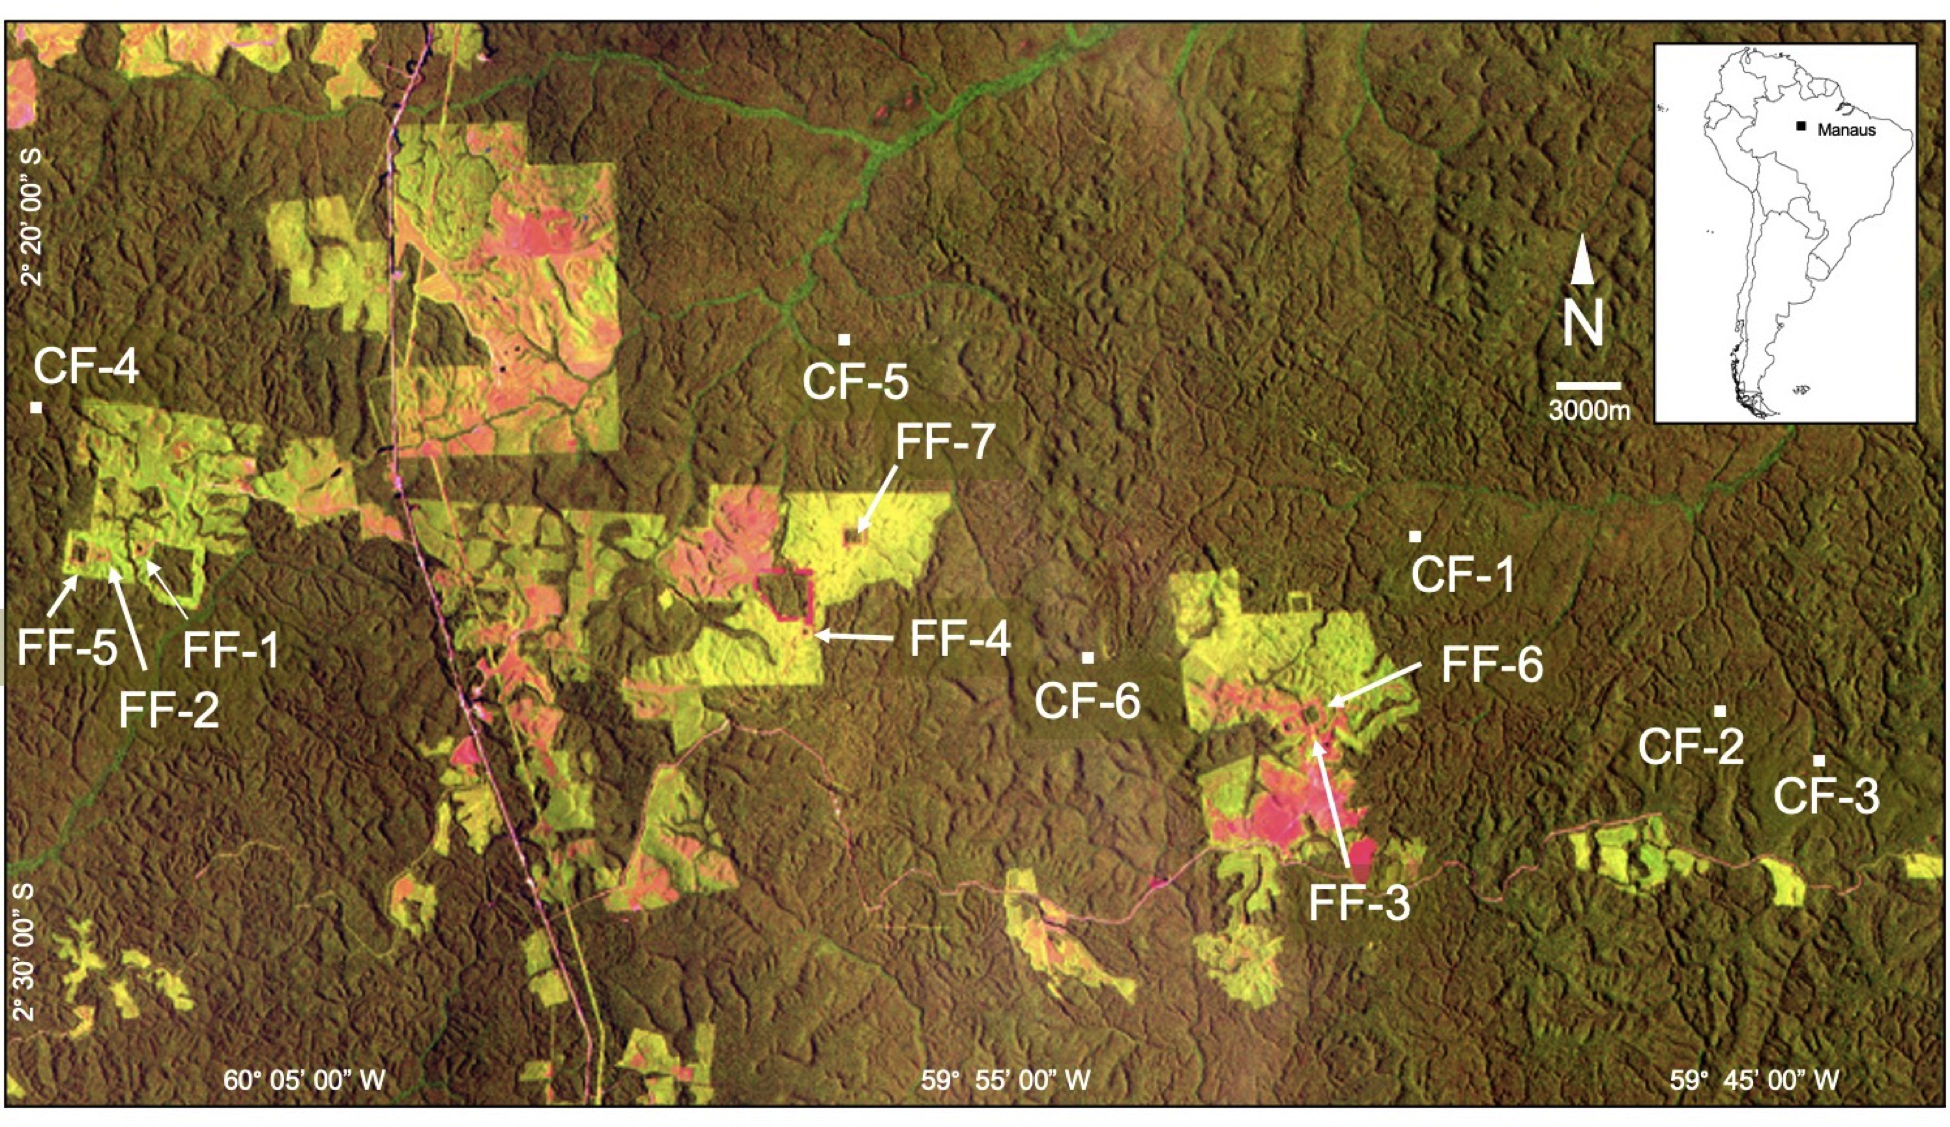
\includegraphics[width=1\linewidth]{Bruna_etal_MetadataS1_files/figure-latex/map-1} \caption{Satellite image of the Biological Dynamics of Forest Fragments Project (ca. 1995) showing the location of the \textit{Heliconia} Demographic Plots. Plots are located in Continuous Forest (CF1-CF6) or Forest Fragments (FF1-FF7), both of which are dark green. Light green areas are regenerating forest, while red indicates pasture. The BDFFP is located ~70 km north of Manaus, Brazil (inset map). For additional details on each plot see Table 1.}\label{fig:map}
\end{figure}

\newpage

\begin{figure}[h]

{\centering 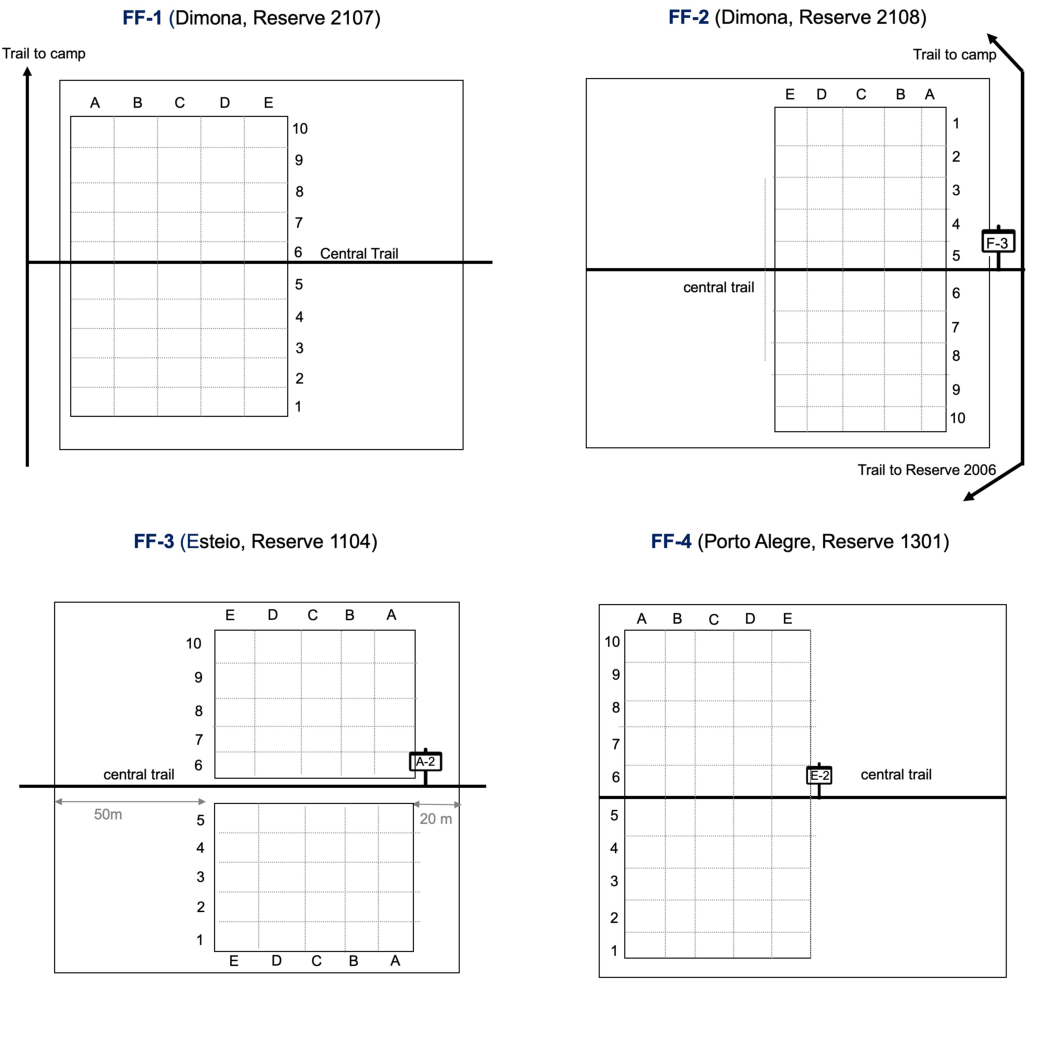
\includegraphics{Bruna_etal_MetadataS1_files/figure-latex/plotsone-1} 

}

\caption{Schematic of the \textit{Heliconia} Demographic Plots in the BDFFP 1-hectare forest fragment reserves. Note: not to scale.}\label{fig:plotsone}
\end{figure}

\newpage
\begin{figure}[h]

{\centering 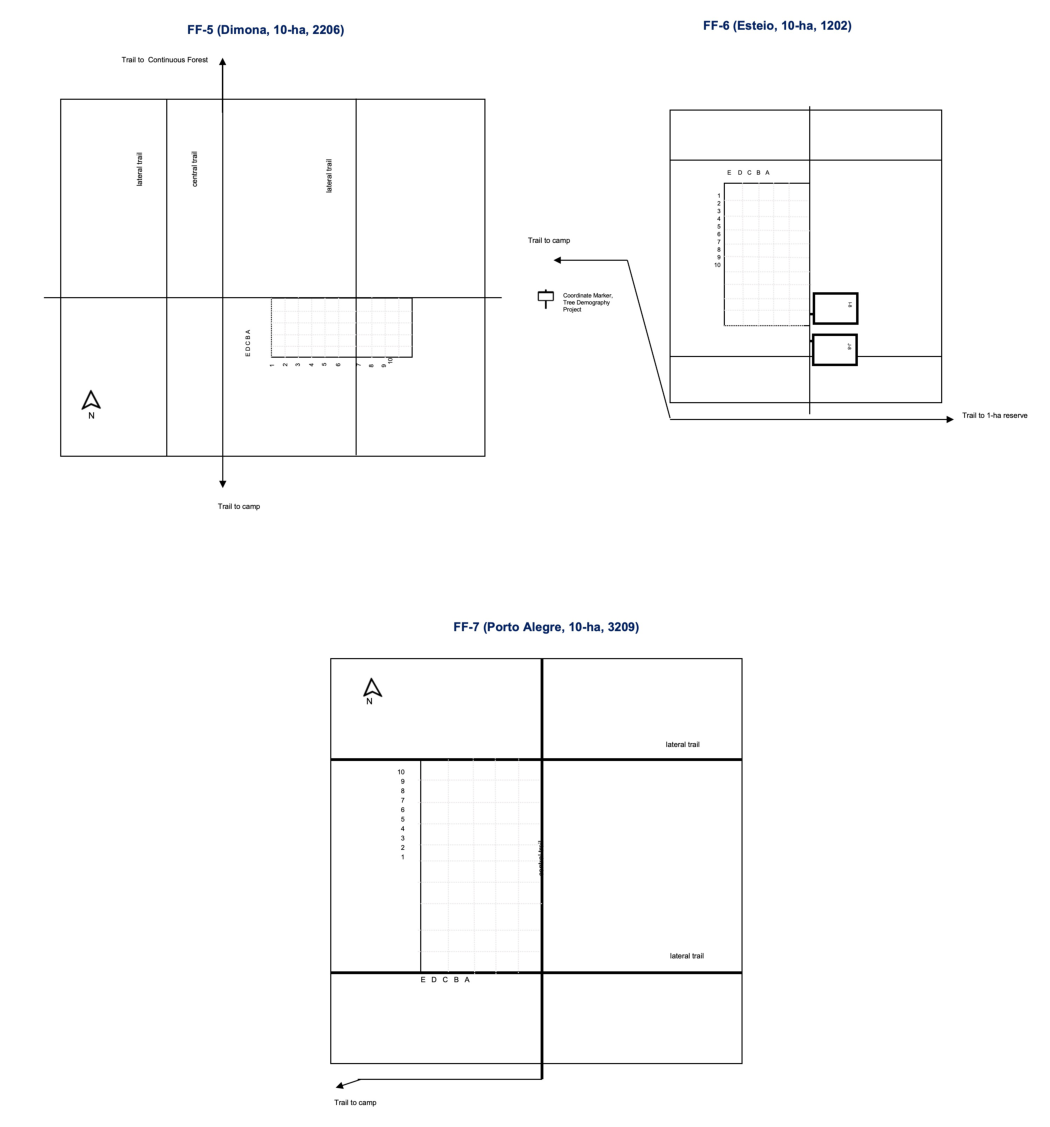
\includegraphics{Bruna_etal_MetadataS1_files/figure-latex/plotsten-1} 

}

\caption{Schematic of the \textit{Heliconia} Demographic Plots in the BDFFP 10-ha forest fragment reserves. Note: not to scale.}\label{fig:plotsten}
\end{figure}
\newpage
\begin{figure}[h]

{\centering 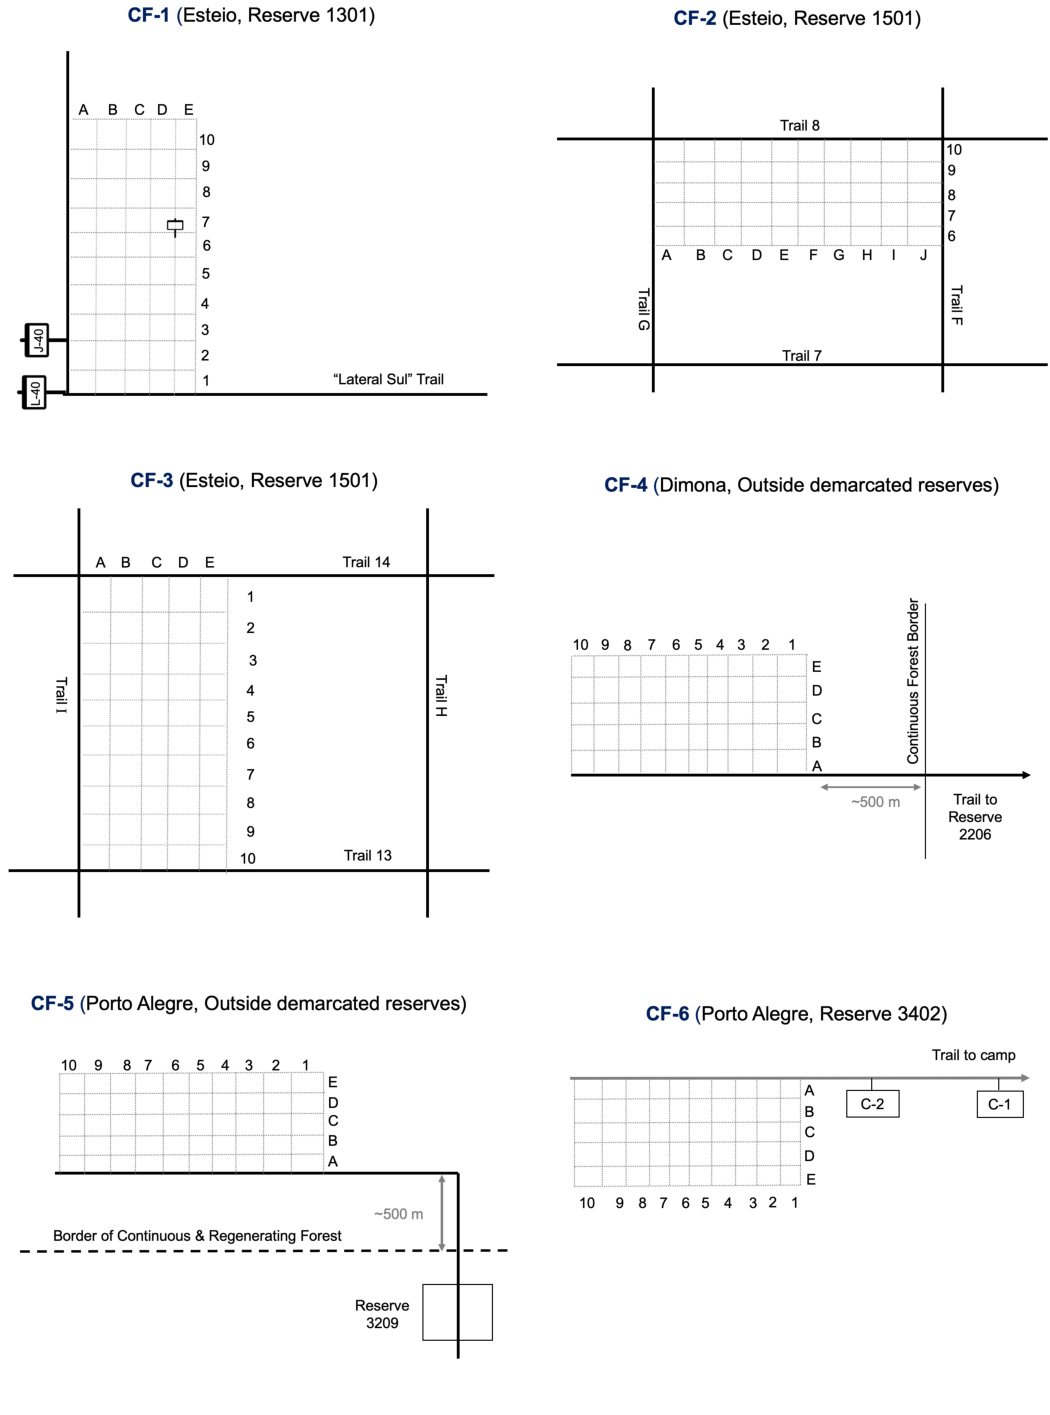
\includegraphics{Bruna_etal_MetadataS1_files/figure-latex/plotscf-1} 

}

\caption{Schematic of each \textit{Heliconia} Demographic Plot in the BDFFP Continuous Forest reserves. Note: not to scale.}\label{fig:plotscf}
\end{figure}
\newpage

\newpage
\blandscape
\nolinenumbers

\textbf{Table 1}. Variable Information for ``Data set File 1: \emph{Descriptors of demographic plots}''.
\renewcommand{\arraystretch}{0.5}

\begin{table}
\centering
\begin{threeparttable}
\begin{tabular}{>{\raggedright\arraybackslash}p{6em}>{\raggedright\arraybackslash}p{19em}>{\raggedright\arraybackslash}p{17em}>{\raggedright\arraybackslash}p{3em}}
\toprule
\textbf{Variable} & \textbf{Definition} & \textbf{Codes} & \textbf{Storage}\\
\midrule
plot & Code used to identify a plot & FF1-FF7: plots in fragments
  
CF1-CF6: plots in continuous forest & string\\
\midrule
habitat & Habitat in which a plot is located & one: 1-ha fragment
  
ten: 10-ha fragment
  
forest: continuous forest & string\\
\midrule
ranch & Ranch in which a plot is located & porto alegre, esteio, dimona & string\\
\midrule
bdffp\_no & BDFFPs Reserve ID Number$^{1}$ & 1104, 1202, 1301, 1501, 2107, 2108, 2206, 3209, 3402, NA & string\\
\midrule
yr\_isolated & For fragments, the year initially isolated & 1980, 1983, 1984 & integer\\
\bottomrule
\end{tabular}
\begin{tablenotes}
\item[1] See Gascon and Bierregaard (2001) for details of the reserve numbering scheme. `NA` indicates the plot is not inside a formally demarcated BDFFP reserve.
\end{tablenotes}
\end{threeparttable}
\end{table}

\newpage

\textbf{Table 2}. Variable Information for ``Data set File 2: \emph{Heliconia Demographic Data}''.
\renewcommand{\arraystretch}{0.5}

\begin{longtable}[l]{>{\raggedright\arraybackslash}p{8em}>{\raggedright\arraybackslash}p{15em}>{\raggedright\arraybackslash}p{19em}>{\raggedright\arraybackslash}p{3em}}
\toprule
\textbf{Variable} & \textbf{Definition} & \textbf{Codes or Range of Values} & \textbf{Storage}\\
\midrule
\endfirsthead
\multicolumn{4}{@{}l}{\textit{(continued)}}\\
\toprule
\textbf{Variable} & \textbf{Definition} & \textbf{Codes or Range of Values} & \textbf{Storage}\\
\midrule
\endhead

\endfoot
\bottomrule
\multicolumn{4}{l}{\rule{0pt}{1em}\textsuperscript{1} For the arrangment of the subplots see Figures 2-4}\\
\endlastfoot
plot & Plot in which plant is located & FF1-FF7, CF1-CF6 & string\\
\midrule
subplot & Subplot in which plant is located & A1-E10 except in CF3, where F6-J10$^{1}$ & string\\
\midrule
plant\_id & Unique ID no. assigned to plant & range = 1-8660 (units: number, precision: 1) & integer\\
\midrule
year & Calendar year of survey & range = 1998-2009 (units: year, precision: 1) & integer\\
\midrule
shts & No. of shoots when surveyed & range = 0-24 (units: shoots, precision: 1) & integer\\
\midrule
ht & Plant height when surveyed & range = 0-226 (units: cm, precision: 1) & integer\\
\midrule
infl & No. of inflorescences (if flowering) & range = 1-7 (units: shoots, precision: 1) & integer\\
\midrule
recorded\_sdlg & New seedling & TRUE, FALSE & logical\\
\midrule
found\_without\_tag & Established (i.e., post-seedling) individual without tag & TRUE, FALSE & logical\\
\midrule
treefall\_status & Plant under fallen tree crowns, branches, or leaf litter & branch: under fallen tree limbs
  
tree: under tree crown or fallen trees
  
litter: under accumulated leaf-litter & string\\
\midrule
census\_status & Plant status in a census & measured: alive, measured
  
dead: died prior to census
  
missing: not found during census & string\\*
\end{longtable}

\elandscape


\clearpage
\renewcommand{\listfigurename}{Figure captions}


\end{document}
